\documentclass{article}

\usepackage{amsmath} % for \text
\usepackage{amssymb} % for \mathbb
\usepackage{amsthm} % for proof environment
\usepackage{hyperref} % for \autoref
\usepackage{cleveref} % for \cref
\usepackage{tikz} % for tikzpicture
\usepackage{graphicx} % for \includegraphics
\usepackage{subcaption} % for subfigure
\usepackage{float} % for H in figure
\usepackage{geometry} % for \newgeometry
\usepackage{fullpage} % for fullpage


\geometry{left = 1.8cm, right = 1.8cm}

\begin{document}

\begin{center}
    \textbf{\LARGE{Ecole Normale Supérieure de Paris-Saclay}}\\
\end{center}

\vspace{1cm}

\begin{center}
    \textbf{Rapport TER}
\end{center}

\noindent\rule{\textwidth}{0.6mm}
\bigskip
\begin{center}
    \textbf{\LARGE{TER - Voiture autonomes avec apprentissage par renforcement et lidar}}
\end{center}
\bigskip
\noindent\rule{\textwidth}{0.6mm}

\bigskip
\begin{center}
    \textsc{Miquel Hugo}
\end{center}
\begin{center}
    \textsc{Plus Basile}
\end{center}

\begin{figure}[b]
    \centering
    \begin{minipage}[h]{0.45\textwidth}
        \raggedright
        
\includegraphics[width=0.6\textwidth]{Images/Logo-ENS-Paris-Saclay.png}
    \end{minipage}
    \begin{minipage}[h]{0.45\textwidth}
        \raggedleft
        
\includegraphics[width=0.6\textwidth]{Images/Logo-Universite-Paris-Saclay.jpg}
    \end{minipage}
\end{figure}


\newpage

\tableofcontents

\newpage

\section{Introduction}

\subsection{Contexte}

Les voitures autonomes sont un sujet de recherche très actif depuis quelques années. 
En effet, elles pourraient révolutionner le monde des transports en permettant de réduire les accidents de la route, 
de diminuer la consommation d'énergie et de réduire les embouteillages. 
Cependant, il reste encore de nombreux défis à relever pour que les voitures autonomes soient utilisées à grande échelle.
En particulier, il est nécessaire de développer des algorithmes d'apprentissage par renforcement qui permettent à une 
voiture autonome d'apprendre à conduire de manière autonome.

\subsection{Objectif et travail réalisé}
L'objectif de ce TER est de développer un algorithme d'apprentissage par renforcement qui permet à une 
voiture RC au format $1/10^{\text{ème}}$ de conduire de manière autonome sur un circuit. Dans un premier temps, nous 
avons utilisé Webots pour la simulation, gym et stable baselines pour l'apprentissage par renforcement.
Dans un second temps, nous avons transféré le réseau de neurones du simulateur à la voiture réelle.
La voiture est équipée d'un lidar qui permet de mesurer la distance entre la voiture et les murs du circuit.

\vspace{0.5cm}
\noindent
Note: Presenter Webots, la voiture réelle, la voiture sur simulateur, le lidar, le circuit etc...


\subsection{L'apprentissage par renforcement}
L'apprentissage par renforcement est une méthode d'apprentissage automatique qui permet à un agent 
d'apprendre à prendre des décisions en interagissant avec un environnement. 

\begin{figure}[H]
    \centering
    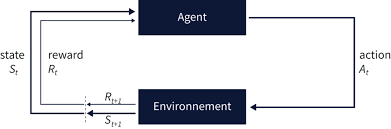
\includegraphics[width=0.6\textwidth]{Images/RL.png}
    \caption{Schéma de l'apprentissage par renforcement}
\end{figure}

\noindent
L'agent prend des actions dans l'environnement et reçoit une récompense en fonction de l'action qu'il a prise. 
L'objectif de l'agent est de maximiser la somme des récompenses qu'il reçoit au cours des itérations. 

\section{Simulation}

\subsection{Webots}

Webots est un logiciel de simulation de robotique développé par Cyberbotics. Il permet de simuler des robots dans un 
environnement 3D. 

\section{Simulation to real world}

\subsection{Transfert du réseau de neurones}

\section{Résultats}

\section{Conclusion}


\end{document}